\chapter{Modelling DISFA} \label{sec:model}
  This chapter describes the path taken in constructing the autoencoding classifier (AEC) network, detailing
  the experiments which were performed to create the final configuration.
  The most important metric used to judge a network in the chapter is the Average ROC score of the classifier
  when applied to the un-seen validation set\footnote{}, the secondary metric will be the error
  in the reconstructed image outputted from the autoencoder. The overall aim is to
  find a configuration where improving the secondary metric (the autoencoder) improves
  the primary metric (the classifier) and that the presence of the autoencoder improves
  the performance of the classifier.

  The results will show, that it is unclear if there is a direct relationship, nonetheless
  the work is a detailed exploration of how autoencoders and classifiers interact with each other
  under various initial preprocessing setups and different autoencoder transfer functions \footnote{These describe the degree to which
  each cost function is trained during training, section \ref{sec:autoalpha} details this in full.}.

  \section{Experimental set up}
    In order to develop the network for modelling the DISFA dataset a set of common
    parameters for experimentation are useful to define, these are shown in table \ref{tab:common}

    \begin{table}[!h]
      \centering { \footnotesize \label{my-label}
      \begin{tabular}{ll}
        \hline
        \textbf{Parameter}                       & \textbf{Value}                \\ \hline
        Optimizer                                & Adam                          \\
        Learning Rate                            & 0.001                         \\
        L2 Regularisation Coefficient            & 0.0                           \\
        Hidden layer activation functions         & ReLu                          \\
        Image downscaling                        & 0.4                           \\
        AU's present                             & 1,2,4,5,6,9,12,15,17,20,25,26 \\
        Iterations:                              & 1000                          \\
        Early model save percent                 & 50\%                          \\
        Weight tensor initial standard deviation & 0.001                         \\
        Bias tensor initial value                & 0.01                          \\
        Validation batch size                    & 500                           \\
        Penultimate fully connected layer size   & 3000                          \\
        \hline
      \end{tabular}
      \caption{Common parameters for most experiments in the section. These parameters should be
      assumed in proceeding sections unless otherwise stated.} \label{tab:common} }
    \end{table}


  % A single hidden layer
  % A single hidden layer
  % A single hidden layer
  % A single hidden layer
  \section{A single hidden layer}
    \begin{table}[h!]
    \centering
    {\footnotesize
    \begin{tabular}{|lllllllll|}
    \hline
    \multicolumn{1}{|l|}{Element} & Type     & \multicolumn{1}{l|}{Dimensions}                     & Type     & \multicolumn{1}{l|}{Dimensions}                      \\ \hline
    \multicolumn{1}{|l|}{x}       &          & \multicolumn{1}{l|}{$47\times47\times1$}            &          & \multicolumn{1}{l|}{}                                \\ \hline
    \multicolumn{1}{|l|}{$L_1$}   & fc       & \multicolumn{1}{l|}{$2209\times14$}              & Binary Softmax & \multicolumn{1}{l|}{$3000\times2\times12$}        \\
    \multicolumn{1}{|l|}{$y_1$}   & dropout  & \multicolumn{1}{l|}{$14$}                         &          & \multicolumn{1}{l|}{$24$}                              \\ \hline
    \multicolumn{1}{|l|}{$L_2$}   & fc       & \multicolumn{1}{l|}{$14\times2209$}              &          & \multicolumn{1}{l|}{}                                   \\
    \multicolumn{1}{|l|}{$y_2$}   &          & \multicolumn{1}{l|}{$3000$}                         &          & \multicolumn{1}{l|}{}                                \\ \hline
    \multicolumn{1}{|l|}{$L_3$}   & reshape & \multicolumn{1}{l|}{}                    &          & \multicolumn{1}{l|}{}                                \\
    \multicolumn{1}{|l|}{$y_3$}   &          & \multicolumn{1}{l|}{$47\times47\times 1$}          &          & \multicolumn{1}{l|}{}                                \\ \hline
    \end{tabular}

    \caption{} \label{net:simple1}

    }
    \end{table}
    %ID = 4 date = '2016_08_14' group = 'alpha'
    As an introduction to the types of results that will be used to evaluate various
    models, this section shows the performance of a neural network with one
    hidden layer. This also should provide a worst case for classification and autoencoding performance.

    The structure of this network is shown in table \ref{net:simple1}, 14 neurons
    are chosen heuristically as there are 14 AU's and one might naively hope that the number of
    neurons required in the hidden layer would be equal to the number of features. Per subject face normalisation
    is chosen from section \ref{sec:meanface} and the images are scaled to be size $118 \times 118$.
    Figure \ref{fig:simple} shows the losses during training, on the train and validation set where table \ref{tab:splitting}
    describes the way the data is partitioned. Overfitting to the train set is evident very early in the training, there are two
    possible reasons, firstly the validation set might be too small to represent all AU's and secondly the model is still quite basic.
    Training the classifier reduces the performance of the autoencoder visibily.

    \begin{table}[h!]
      \centering
      {\footnotesize
      \begin{tabular}{|l|l|}
      \hline
      set & subjects   \\
      \hline
       Train          & 2,4,6,8,10,12,16,18,23,25,27,29,31      \\
      \hline
      Test      & 1,3,5,7,9,11,13,17,21,24,26,28,30,32 minus validation set     \\
      \hline
      Validation           & 500 chosen randomly taken from test set      \\
     \hline
      \end{tabular}
      \caption{Typical split of the DISFA dataset for experimentation perposes}
      \label{tab:splitting}  }
    \end{table}


    \begin{figure}[!h]
    \centering
    \includegraphics[width =\hsize]{../graphs/losses_2016_08_14_004.pdf}
    \caption{The losses of a neural network consisting of a $118^2$ neuron input layer, a 14
    neuron hidden layer, a branch of the same size as the input layer for autoencoding
    and branches for binary softmax classifiers for each AU. The classifier mean
    squared loss is shown only for interest, the network trains by minimising
    the cross entropy. The $\alpha$ coefficient determines the balance between the
    classifier and the autoencoder losses, $\alpha=1$ signifies only autoencoder training
    while $\alpha=0$ means only classifier training. Overfitting is observed
    on all loss functions. Training the classifier
    overwrites the weights and hence ends up reducing
    the performance of the autoencoder.}
    \label{fig:simple}
    \end{figure}

    \begin{table}[!h]
    \centering
    {\small
    \begin{tabular}{llllll}
    \hline
    \textbf{Class}    & \textbf{ROC} & \textbf{ROC} & \textbf{Max F1} & \textbf{Max Percision} & \textbf{Max Recall} \\ \hline
    1                 & 0.5          & fail         & 0.09            & 0.06                   & 1.0                 \\
    2                 & 0.6          & poor         & 0.07            & 0.05                   & 1.0                 \\
    4                 & 0.62         & poor         & 0.31            & 0.27                   & 1.0                 \\
    5                 & 0.49         & fail         & 0.02            & 0.02                   & 1.0                 \\
    6                 & 0.8          & fair         & 0.48            & 0.42                   & 1.0                 \\
    9                 & 0.46         & fail         & 0.11            & 0.06                   & 1.0                 \\
    12                & 0.89         & good         & 0.67            & 0.73                   & 1.0                 \\
    15                & 0.46         & fail         & 0.11            & 0.06                   & 1.0                 \\
    17                & 0.55         & fail         & 0.18            & 0.25                   & 1.0                 \\
    20                & 0.51         & fail         & 0.09            & 0.12                   & 1.0                 \\
    25                & 0.65         & poor         & 0.51            & 0.42                   & 1.0                 \\
    26                & 0.57         & fail         & 0.32            & 0.23                   & 1.0                 \\ \hline
    \textbf{Average:} & 0.59         & fail         & 0.25            & 0.22                   & 1.0                 \\ \hline
    \end{tabular} }
    \caption{}
    \label{my-label}
    \end{table}


    \newpage
    %
    %
    %
    %
  \section{Joint classification}

    Typical deep neural networks are used to classify
    one image into only one category. The case with the DISFA dataset is different, we
    would like to be able to classify the categories jointly,  putting one frame into more than
    one AU category. Ideally the network would output a confidence score between 0 and 1
    to signfy if an AU is present and we would calculate some optimum threshold value
    (ideally this would be 0.5).

    The following list details three possible solutions to the joint classification problem:

    \begin{itemize} \label{sec:binsoft}
      \item {\bf Softmax Layer} - This is a traditional, fully connected layer with
                                  a softmax activation function (see equation \ref{eq:softmax}).
                                  The issue with this is that it provides a probability distribution over AUs
                                  but the required quantity is a probability distribution for each AU. In the implementation
                                  the negative neuron of each binary layer is only used for training perposes, and it is
                                  discarded while evaulating the classification performance.
      \item {\bf Sigmoid Layer} - This again is like the previous solution but instead each neuron gives a confidence
                                  score between 0 and 1 for each AU with a sigmoid function (see equation \ref{eq:sigmoid}).
                                  The issue with this however is that sigmoid
                                  functions have vanishing gradients at large input values
                                  hence training may become difficult.
      \item {\bf Binary Softmax Layers} - Here there is a two neuron softmax layer
                                          for each AU, this doubles the amount of weights
                                          but gives a probability over the presence and
                                          absence of each AU which is ideal.
    \end{itemize}

    Table \ref{net:classcompnet} compares how each of these solutions perform using the network described in
    tables \ref{net:classcompnet}, this network was chosen because it contains all of the main
    components of larger networks typically used for classification tasks, such as a convolutional
    layer, max pool layer and fully connected layer. It contains the autoencoder section which will be
    explored later on in the section mainly out of interest.

    \begin{table}[h!]
    \centering
    {\footnotesize
    \begin{tabular}{|lllllllll|}
    \hline
    \multicolumn{1}{|l|}{Element} & Type     & \multicolumn{1}{l|}{Dimensions}                     & Type     & \multicolumn{1}{l|}{Dimensions} \\ \hline
    \multicolumn{1}{|l|}{x}       &          & \multicolumn{1}{l|}{$47\times47\times1$}            &          & \multicolumn{1}{l|}{}          \\ \hline
    \multicolumn{1}{|l|}{$L_1$}   & conv 1   & \multicolumn{1}{l|}{$5\times 5\times1\times 64$}    &          & \multicolumn{1}{l|}{}          \\
    \multicolumn{1}{|l|}{$y_1$}   &          & \multicolumn{1}{l|}{$43\times43\times64$}           &          & \multicolumn{1}{l|}{}          \\ \hline
    \multicolumn{1}{|l|}{$L_2$}   & max pool & \multicolumn{1}{l|}{$2\times 2$}                    &          & \multicolumn{1}{l|}{}          \\
    \multicolumn{1}{|l|}{$y_2$}   &          & \multicolumn{1}{l|}{$22\times22\times 64$}          &          & \multicolumn{1}{l|}{}          \\ \hline
    \multicolumn{1}{|l|}{$L_3$}   & fc       & \multicolumn{1}{l|}{$30976\times3000$}              & \multicolumn{2}{l|}{Sotmax Layer or}      \\
    \multicolumn{1}{|l|}{$y_3$}   &          & \multicolumn{1}{l|}{}                               & \multicolumn{2}{l|}{Sigmoid Layer or}     \\
    \multicolumn{1}{|l|}{$L_4$}   & dropout  & \multicolumn{1}{l|}{$3000$}                         & \multicolumn{2}{l|}{Binary Softmax Layer} \\
    \multicolumn{1}{|l|}{$y_4$}   &          & \multicolumn{1}{l|}{}                               &          & \multicolumn{1}{l|}{}          \\ \hline
    \multicolumn{1}{|l|}{$L_5$}   & resize\& reshape & \multicolumn{1}{l|}{$2$}                    &          & \multicolumn{1}{l|}{}          \\
    \multicolumn{1}{|l|}{$y_5$}   &          & \multicolumn{1}{l|}{$43\times43\times 64$}          &          & \multicolumn{1}{l|}{}          \\ \hline
    \multicolumn{1}{|l|}{$L_6$}   & deconv 1   & \multicolumn{1}{l|}{$5\times 5\times1\times 64$}  &          & \multicolumn{1}{l|}{}\\
    \multicolumn{1}{|l|}{$y_6$}   &          & \multicolumn{1}{l|}{$47\times47\times1$}            &          & \multicolumn{1}{l|}{}         \\ \hline
    \end{tabular}

    \caption{Set up for deciding on which final layer structure to use.
    This network is very similar to \textbf{Network 1} which is described later in the section.} \label{net:classcompnet}

    }
    \end{table}


    \begin{table}[!h] {\small
      \centering
      \begin{tabular}{lccc}
      \hline
      Final Layer   & Av. ROC &   Av. Best F1 &   Autoencoder Loss (Not normalised) \\
      \hline
      Binary Softmax Layers  &   0.73 &  0.34 &   20.7 \\
      Softmax Layer          &   0.69 &  0.30 &   15.8 \\
      Sigmoid Layer          &   0.50 &  0.19 &  126.2 \\
      \hline
      \end{tabular}
    \caption{Comparison of the three ways the final layer could be implemented using network 1 (see table \ref{compnet})} \label{net:classcompnet} }
    \end{table}

    The results show that the binary softmax layer outperforms the other solutions. The
    softmax layer is only slightly worse, but in order to accomodate for the potential of higher rates
    it is clear that the binary softmax is the better choice. This is because, in joint classification problems
    the simple softmax layer struggles to report more than 2 AU's as the outputs must add up to one.
    The low performance of the softmax layer is interesting and one reason might be that of vanishing gradients due to
    the bottleneck layer containing high activation values.

    As the softmax layer is better in the results and has a better potential for good results
    it is chosen as the classifier for the rest of this work.

  % Autoencoder classifier branching and balancing
  % Autoencoder classifier branching and balancing
  % Autoencoder classifier branching and balancing
  % Autoencoder classifier branching and balancing
  \section{Autoencoder classifier balancing} \label{sec:autoalpha}
    A key structure that is to be investigated in this report is a network with two objective functions:
    autoencoder and classifier. This is achieved by having a bottleneck layer where the branching occurs.
    The autoencoder has symmetry along this bottleneck, while the classifier consists of one further layer
    (the binary softmax classifier from the previous section). The cost function for the whole network is as follows:

    \begin{equation}
        J(\tilde{\mathbf{x}},\tilde{\mathbf{y}}) = -\frac{1-\alpha(t)}{2FN}\tilde{\mathbf{y}}\cdot\log(\mathbf{y}(\tilde{\mathbf{x}}))
        + \frac{\alpha(t)}{N}\left |\mathbf{y}(\tilde{\mathbf{x}}) \odot \mathbf{M}-\tilde{\mathbf{x}}\right | ^2
    \end{equation}

    Here F is the number of AU's, N is the size of the batch and $\alpha(t)$ is a
    function which balances the two costs. $\alpha(t)$ might be constant $\left ( \alpha_{\text{constant}}(t)=\frac{1}{2} \right )$ or
    some sort of polynomial which stays in the range $[0,1]$.

    For much of the initial investigations we employ:
    \begin{equation}
    \alpha_{\text{step}}(t,p,T) =
    \begin{cases}
      1           & \text{if}\ t<pT \\
      0           & \text{otherwise}
    \end{cases}
    \end{equation}

    Where t indexes iterations, T is the total number of iterations and p is the
    percentage of iterations that should be in the first region of the piecewise function
    where $\alpha=1$.
    This nicely expresses what is typically meant by pre-training in the literatue, it trains
    the autoencoder up until iteration $pT$ (normally $p=\frac{1}{2}$ or $p=\frac{2}{3}$) and then the classifier for the remainder of the time.
    This acts as a good base case to test both sides of the network, later more interesting
    functions will be explored such as the sigmoid step:

    \begin{equation}
      \alpha_{\text{sigmoid}}(t,T,p,\tau) = \frac{1}{1 + \exp(1 + \tau (t/T - p))}
    \end{equation}

    Or a polynomial function:

    \begin{equation}
      \alpha_{\text{poly}}(t,T,n) = 1 - \left ( \frac{t}{T} \right )^n
    \end{equation}

    Examples of such functions are plotted in the following figure:

    \begin{figure}[!h]
    \centering
    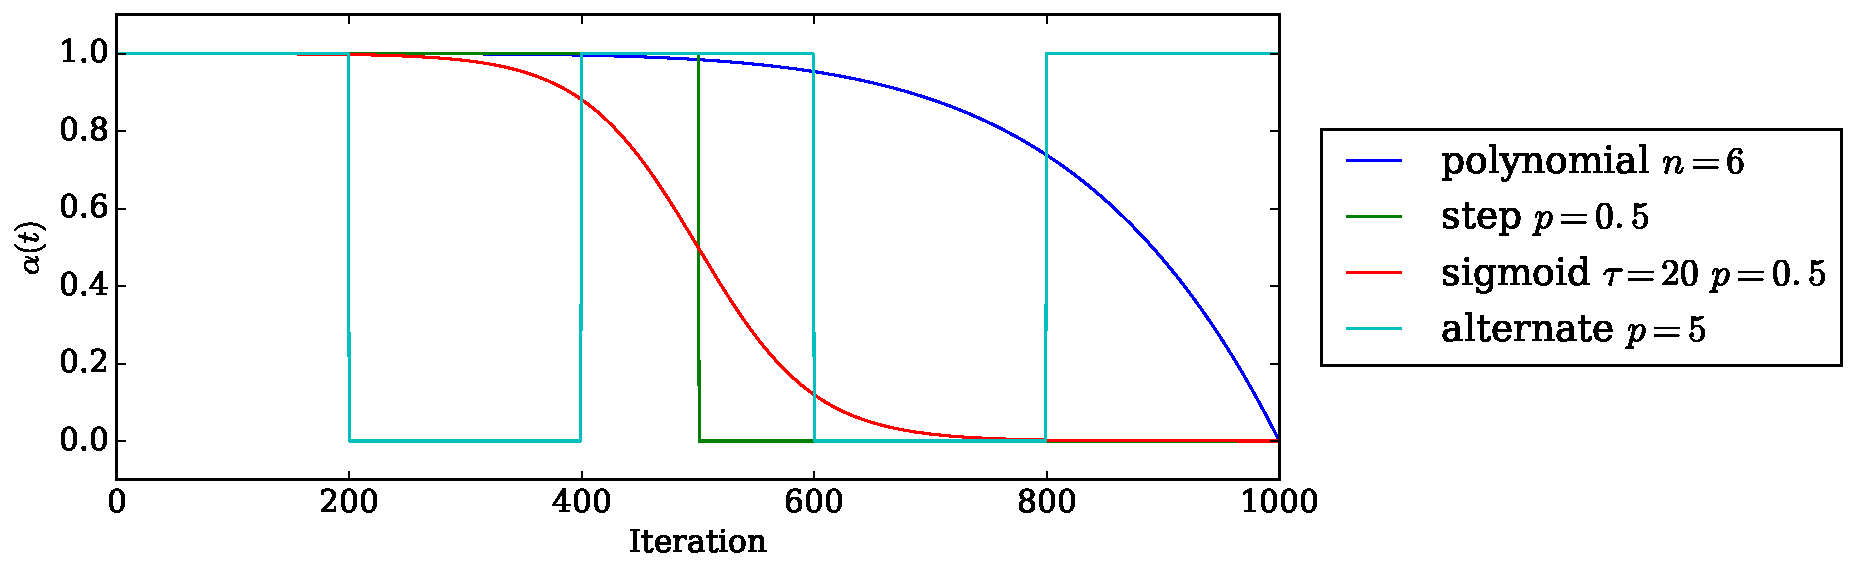
\includegraphics[width =\hsize]{figures/alpha.pdf}
    \caption{Examples of alpha functions described in section \ref{sec:autoalpha}
    for the polynomial case higher values of $n$ decrease the amount of training
    the classifier recieves. While in the case of the step p dictates the training
    that each network recieves, the sigmoid can be seen as a smoothed out step function
    with the two being equivalent as $ \tau \rightarrow \infty$. Similarly as $n \rightarrow \infty$
    the polynomial function turns into a constant function with $c=1$ except at the final
    iteration.}
    \label{fig:alpha_functions}
    \end{figure}

    % def alpha_sigmoid(_x,_N,a=20,b=0.5):
    %     x = float(_x)
    %     N = float(_N)
    %     arg = x/N - b
    %     return 1.0/(1.0 + exp(a*arg))

  %
  %
  %
  %
  %
  \section{Convolutional Networks}

    Now that some basic structures have been tested we proceed to convolutional networks,
    inspired by the literature (see table \ref{compnet}) 3 networks are defined. Network 2 is shown in table \ref{compnet}, Network 3
    adds another convolutional layer of size $5\times 5 \times 64 \times 64$ and Network 4 adds a $4\times 4 \times 64 \times 128$ layer
    on top of Network 3. Regarding the decoder section of the inverse operations are performed, see appendix \label{appendix1} for full details
    for networks 1,2,3 and 4.

    % network.append(cnn_layer(ll(network), [5, 5, 64, 64], 'VALID', 'Convolution_2', config, act=act))
    % network.append(cnn_layer(ll(network), [4, 4, 64, 128], 'VALID', 'Convolution_3', config, act=act))

    \begin{table}[h!] \caption*{\textbf{Network 2}}
    \centering
    {\footnotesize
    \begin{tabular}{|lllllllll|}
    \hline
    \multicolumn{1}{|l|}{Element} & Type     & \multicolumn{1}{l|}{Dimensions}                     & Type     & \multicolumn{1}{l|}{Dimensions}  \\ \hline
    \multicolumn{1}{|l|}{x}       &          & \multicolumn{1}{l|}{$47\times47\times1$}            &          & \multicolumn{1}{l|}{}            \\ \hline
    \multicolumn{1}{|l|}{$L_1$}   & conv 1   & \multicolumn{1}{l|}{$5\times 5\times1\times 64$}    &          & \multicolumn{1}{l|}{}            \\
    \multicolumn{1}{|l|}{$y_1$}   &          & \multicolumn{1}{l|}{$43\times43\times64$}           &          & \multicolumn{1}{l|}{}            \\ \hline
    \multicolumn{1}{|l|}{$L_2$}   & max pool & \multicolumn{1}{l|}{$2\times 2$}                    &          & \multicolumn{1}{l|}{}            \\
    \multicolumn{1}{|l|}{$y_2$}   &          & \multicolumn{1}{l|}{$22\times22\times 64$}          &          & \multicolumn{1}{l|}{}            \\ \hline
    \multicolumn{1}{|l|}{$L_3$*}   & fc       & \multicolumn{1}{l|}{$30976\times3000$}              & Binary
                                                                                                      Softmax & \multicolumn{1}{l|}{$3000\times2\times12$}        \\
    \multicolumn{1}{|l|}{$y_3$}   & dropout  & \multicolumn{1}{l|}{$3000$}                         &          & \multicolumn{1}{l|}{$24$}        \\ \hline
    \multicolumn{1}{|l|}{$L_4$}   & fc       & \multicolumn{1}{l|}{$3000\times30976$}              &          & \multicolumn{1}{l|}{}            \\
    \multicolumn{1}{|l|}{$y_4$}   &          & \multicolumn{1}{l|}{$3000$}                         &          & \multicolumn{1}{l|}{}            \\ \hline
    \multicolumn{1}{|l|}{$L_5$}   & resize\& reshape & \multicolumn{1}{l|}{$2$}                    &          & \multicolumn{1}{l|}{}            \\
    \multicolumn{1}{|l|}{$y_5$}   &            & \multicolumn{1}{l|}{$43\times43\times 64$}          &          & \multicolumn{1}{l|}{}            \\ \hline
    \multicolumn{1}{|l|}{$L_6$}   & deconv 1   & \multicolumn{1}{l|}{$5\times 5\times1\times 64$}  &          & \multicolumn{1}{l|}{}            \\
    \multicolumn{1}{|l|}{$y_6$}   &            & \multicolumn{1}{l|}{$47\times47\times1$}            &          & \multicolumn{1}{l|}{}             \\ \hline
    \end{tabular}

    \caption{A network used many times in the report, for further details see appendix \ref{appendix1} \label{compnet}
    \newline *Bottleneck layer}
    }
    \end{table}

    %
    %
    %
    %
    %
    \subsection{Preprocessing methods} \label{sec:psearch}

      With the goal of creating the AEC network we performed a search on some hyperparameters
      including the preprocessing method from section \ref{sec:methods} and on the 4 main activation functions
      that are typically used on the last layer of an autoencoder, table \ref{tab:psearch} shows the results.
      These parameters cover a lot of possible configurations and should have markedly different results, the idea
      is that the encoding at the bottleneck layer should be different for each set of parameters and that
      one of these will offer a good starting set of weights for the classifier to train from.

      \begin{table}[!h] {\small
        \centering
      \begin{tabular}{lllrrrrrr}
            && &   \multicolumn{3}{|c|}{Autoencoder Training} &  \multicolumn{3}{c|}{Classifier Training}    \\
        \hline
         i&Preprocesing    & Activation Function&  ROC&F1&AE Loss & ROC & F1 & AE Loss \\
         \hline
         1&Per Subject Contrast Face & linear &    0.49 &   0.19 &     0.12 &    0.82 &   0.46 &     0.18 \\
         2&Per Subject Contrast Face & tanh   &    0.49 &   0.19 &     0.12 &    0.82 &   0.46 &     0.13 \\
         3&Per Subject Contrast Face & relu   &    0.63 &   0.19 &     0.12 &    0.81 &   0.44 &     0.14 \\
         4& Per Subject Contrast Face & sigmoid &    0.52 &   0.2  &     0.13 &    0.08 &   0.19 &     0.13 \\
         5&Contrast          & linear &    0.40 &   0.19 &     0.19 &    0.74 &   0.34 &     1.46 \\
         6&Contrast          & tanh   &    0.61 &   0.19 &     0.20 &    0.72 &   0.35 &     0.35 \\
         7&Contrast          & relu   &    0.59 &   0.19 &     0.25 &    0.75 &   0.36 &     0.65 \\
         8& Contrast         & sigmoid &    0.54 &   0.19 &     0.22 &    0    &   0.19 &     0.28 \\
         9&Face              & linear &    0.46 &   0.19 &     0.06 &    0.73 &   0.35 &     0.26 \\
         10&Face              & tanh   &    0.52 &   0.19 &     0.08 &    0.74 &   0.35 &     0.13 \\
         11&Face              & relu   &    0.45 &   0.19 &     0.09 &    0.73 &   0.36 &     0.35 \\
         12& Face             & sigmoid &    0.47 &   0.2  &     0.1  &    0.72 &   0.35 &     0.13 \\
         \hdashline
         13&Per Subject Face  & linear &    $0.64$ &   $0.19$ &     $0.03$ &    $0.83$ &   $0.48$ &     $0.12$ \\
         &{\it error:}  &&$\pm$0.02 &$\pm$0.01 &$\pm$0.02  &$\pm$0.02 &$\pm$0.01 &$\pm$0.02 \\
         \hdashline
         14&Per Subject Face  & tanh   &    0.56 &   0.19 &     0.03 &    0.81 &   0.47 &     0.05 \\
         15&Per Subject Face  & relu   &    0.56 &   0.19 &     0.04 &    0.81 &   0.48 &     0.11 \\
         16& Per Subject Face      & sigmoid &    0.62 &   0.23 &     0.04 &    0.81 &   0.46 &     0.05 \\
         17&Range [-1,1]      & linear &    0.50 &   0.19 &     0.07 &    0.73 &   0.35 &     3.90 \\
         18&Range [-1,1]      & tanh   &    0.54 &   0.19 &     0.07 &    0.75 &   0.35 &     0.30 \\
         19&Range [-1,1]      & relu   &    0.48 &   0.19 &     0.15 &    0.73 &   0.35 &     4.73 \\
         20& Range [-1,1]      & sigmoid &    0.49 &   0.2  &     0.12 &    0.73 &   0.31 &     0.36 \\
         21&None              & linear &    0.51 &   0.19 &     0.08 &    0.74 &   0.34 &     4.02 \\
         22&None              & tanh   &    0.59 &   0.19 &     0.07 &    0.71 &   0.33 &     0.93 \\
         23&None              & relu   &    0.53 &   0.19 &     0.20 &    0.53 &   0.23 &     0.41 \\
         24& None       & sigmoid &    0.47 &   0.19 &     0.09 &    0.65 &   0.29 &     0.46 \\
         25&Contrast Face     & linear &    0.56 &   0.19 &     0.24 &    0.74 &   0.35 &     0.40 \\
         26&Contrast Face     & tanh   &    0.54 &   0.19 &     0.24 &    0.75 &   0.38 &     0.26 \\
         27&Contrast Face     & relu   &    0.54 &   0.19 &     0.25 &    0.74 &   0.35 &     0.35 \\
         28& Contrast Face    & sigmoid &    0.44 &   0.19 &     0.25 &    0.71 &   0.34 &     0.26 \\
         \hline
        \end{tabular}
          \caption{Comparison of four activation functions for the autoencoder for each type of preprocessing method.
          No significant difference is seen between the activation functions apart from with the sigmoid
          which makes training the classifier fail competely.
          Error values are required because tensorflow does implement fully determinsitic
          processing with GPU cards (see section \ref{sec:GPU} the values in the errors were
          calculated by rerunning experiment 13 5 times. The autoencoder losses were caluclated
          by first appyling the inverse transform of the preprocessing method and then taking the mean squared
          difference between the reconstructed image and original image. {\bf Experimental Configuration:}
          The alpha function is $\alpha(t)=\alpha_{\text{step}}(t,0.5,1000)$.
          meaning the autoencoder training runs for 500 iterations and then the classifier for 500.
          The network is described in table \ref{compnet} and the training datasets are split in half as in section
          \ref{sec:splitting}.}
      \label{tab:psearch} }
      \end{table}

      The highest ROC and F1 score is found in experiment 13 in table \ref{tab:psearch}. Experiment 12
      has effectively the same score and a lower final autoencoder loss, but it uses the tanh activaition
      function and hence cannot fully reconstruct the input image which has values well outside the
      range $[-1,1]$ hence linear activation function is chosen.

      The network is in quite a different state, looking at the auteoncoder loss
      suggesting there is some degree of cooperation in the earlier experiment.
      The classification rate is also slightly better in the classifier and autoencoder
      training experiment. It may be however that the network is too small to accomodate both
      functions and that this method might allow the training of larger models.
      \newpage
    %
    %
    %
    %
    %
    \subsection{Shared Weights}
      In order to reduce the number of parameters in an autoencoder, to avoid overfitting
      and the probability of learning the identity function, it is often helpful to share weights
      between the encoder and decoder sections. Using the experimentation framework already defined
      checking whether this is worthwhile is easy and insightful to do. Table \ref{tab:sharedweights} shows
      for three networks the effect of having and not having shared weights.

      \begin{table}[!h] \centering
      {\small
      \begin{tabular}{rrllrrrrrrrr}
        &&&&   \multicolumn{3}{|c|}{Autoencoder Training} &  \multicolumn{3}{c|}{Classifier Training}    \\
      \hline
        i & Network               &   Shared Weights &    ROC&F1&AE Loss & ROC & F1 & AE Loss \\
      \hline
       1 & 2    & False     &    0.38 &   0.19 &     0.03 &    0.79 &   0.45 &     0.05 \\
       2 & 2    & True      &    0.48 &   0.19 &     0.02 &    0.81 &   0.48 &     0.12 \\
      \hline
      4 & 3    & False     &    0.55 &   0.19 &     0.03 &    0.78 &   0.41 &     0.06 \\
      5 & 3    & True      &    0.56 &   0.19 &     0.02 &    0.8  &   0.46 &     0.18 \\
      \hline
      8 & 4     & False     &    0.54 &   0.19 &     0.03 &    0.77 &   0.38 &     0.05 \\
      9 & 4     & True      &    0.42 &   0.19 &     0.03 &    0.78 &   0.42 &     1.37 \\
       \hline
      \end{tabular}}\caption{{\bf Experimental Configuration:}
      The alpha function is $\alpha(t)=\alpha_{\text{step}}(t,0.5,1000)$.
      meaning the autoencoder training runs for 500 iterations and then the classifier for 500.
      The network is described in table \ref{compnet} and the training datasets are split in half as in section
      \ref{sec:splitting}.} \label{tab:sharedweights} \end{table}

      It can be seen that using shared weights actually consistently improves the classification
      performance by a small amount and in some cases the autoencoder performance. After the classifier has
      destroyed the autoencoder, as expected, the shared weights cases suffers a much higher loss. This is of course
      because the classifier does not have access to the decoder weights if the weights are not shared and hence
      changes fewer parameters.
    %
    %
    %
    %
    %
    \subsection{Local Contrast Normalisation}

      The local contrast normalisation scheme as described in section \ref{sec:lrn}
      was applied to the three test networks.


      Table \ref{tab:lrn} shows experiments exploring whether these layers improve
      classification performance
      \begin{table}[!h] \centering
      {\small
      \begin{tabular}{rrllrrrrrrrr}
        &&&   \multicolumn{3}{|c|}{Autoencoder Training} &  \multicolumn{3}{c|}{Classifier Training}    \\
      \hline
        i & Network             & LRN Layers   &    ROC&F1&AE Loss & ROC & F1 & AE Loss \\
      \hline
       1 & 2 & 0  &    0.48 &   0.19 &     0.02 &    0.81 &   0.48 &     0.12 \\
       2 & 2 & 1  &    0.49 &   0.19 &     0.02 &    0.81 &   0.47 &     0.13 \\
      \hline
       3 & 3 & 0  &    0.56 &   0.19 &     0.02 &    0.8  &   0.46 &     0.18 \\
       4 & 3 & 1  &    0.57 &   0.19 &     0.02 &    0.8  &   0.46 &     0.19 \\
       5 & 3 & 2  &    0.52 &   0.19 &     0.02 &    0.8  &   0.45 &     0.22 \\
      \hline
       6 & 4 & 0  &    0.42 &   0.19 &     0.03 &    0.78 &   0.42 &     1.37 \\
       7 & 4 & 1  &    0.52 &   0.19 &     0.03 &    0.79 &   0.44 &     1.02 \\
       8 & 4 & 2  &    0.52 &   0.19 &     0.03 &    0.8  &   0.44 &     0.88 \\
      \hline
      \end{tabular}}\caption{Results for applying local contrast normalisation layers
      for the three test networks. {\bf Experimental Configuration:} see caption
      for table \ref{tab:sharedweights}}\label{tab:lrn}  \end{table}

      Table \ref{tab:lrn} shows that for larger networks LRN allows them to compete with
      the smaller ones.

      \newpage
    %
    %
    %
    %
    %
    %
    \subsection{Dropout}
      Varying degrees of (see section \ref{sec:dropout}) were applied to each test network at the bottleneck layer. Table
      \begin{table}[h]
      \centering
      \begin{tabular}{rllrrrrrrrr}
                           &         &                                                                                   &                                                                                  & \multicolumn{1}{r|}{} & \multicolumn{3}{c|}{Autoencoder Training}                          & \multicolumn{3}{c|}{Classifier Training}                           \\ \hline
      i                    & network & \multirow{2}{*}{\begin{tabular}[c]{@{}l@{}}Autoencoder\\ Iterations\end{tabular}} & \multirow{2}{*}{\begin{tabular}[c]{@{}r@{}}Classifier\\ Iterations\end{tabular}} & Dropout                    & ROC                  & F1                   & AE Loss              & ROC                  & F1                   & AE Loss              \\
      \multicolumn{1}{l}{} &         &                                                                                   &                                                                                  & \multicolumn{1}{l}{}  & \multicolumn{1}{l}{} & \multicolumn{1}{l}{} & \multicolumn{1}{l}{} & \multicolumn{1}{l}{} & \multicolumn{1}{l}{} & \multicolumn{1}{l}{} \\ \hline
      1                    & 2       & 1000              & 500     & 1        & 0.49     & 0.19      & 0.02      & 0.8                  & 0.47                 & 0.12                 \\
      2                    & 2       & 1000             & 500       & 0.9      & 0.49     & 0.19      & 0.03      & 0.8                  & 0.47                 & 0.11                 \\
      3                    & 2       & 1000             & 500       & 0.8      & 0.52     & 0.19      & 0.03      & 0.82                 & 0.48                 & 0.08                 \\
      4                    & 2       & 1000             & 1000       & 0.8      & 0.52     & 0.19      & 0.03      & 0.8                  & 0.46                 & 0.11                 \\
      \hline
      5                    & 3       & 1000             & 500       & 1        & 0.51     & 0.19      & 0.02      & 0.81                 & 0.46                 & 0.21                 \\
      6                    & 3       & 1000             & 500       & 0.9      & 0.51     & 0.19      & 0.02      & 0.81                 & 0.46                 & 0.25                 \\
      7                    & 3       & 1000             & 500       & 0.8      & 0.49     & 0.19      & 0.03      & 0.82                 & 0.46                 & 0.13                 \\
      6                    & 3       & 1000             & 1000       & 0.8      & 0.57     & 0.19      & 0.02      & 0.81                 & 0.44                 & 0.33                 \\
      \hline
      9                    & 4       & 1000             & 500       & 1        & 0.6      & 0.19      & 0.03      & 0.78                 & 0.42                 & 1.03                 \\
      10                   & 4       & 1000             & 500       & 0.9      & 0.63     & 0.19      & 0.03      & 0.71                 & 0.35                 & 0.15                 \\
      11                   & 4       & 1000             & 500       & 0.8      & 0.5      & 0.19      & 0.03      & 0.73                 & 0.36                 & 0.08\\
      12                   & 4       & 1000             & 1000       & 0.8      & 0.52      & 0.19      & 0.03      & 0.77   & 0.38     & 1.01\\
      \hline
      \end{tabular}
      \caption{12 experiments which investigate the affect on appyling dropout to the three test networks, autoencoder iterations describes how leftarrow
      the autoencoder is trained for and then classifier iterations describes for how long the classifier is then trained. {\bf Experimental Configuration:} see caption for table \ref{tab:sharedweights}}
      \label{tab:dropout}
      \end{table}

      In networks two and three dropout seems to improve the overall performance of the network. Network three however
      actually performce worse, this could be because it has more parameters and hence requires longer training.


      \newpage
    %
    %
    %
    %
    %
    %
    \subsection{L2 Regularisation}
      L2 Regularisation incurs a penalty to using weights which have high values. This was implemented by adding L2
      loss terms for all weight variables. Experiments shown in table
      \ref{tab:l2_1} were then performed to get an idea of the sensitivy the system has to
      the L2 Coefficient $\beta$, it defines how much effort the training algorithm
      puts into the reducing the L2 loss term. The new cost function becomes:

      \begin{equation}
          J(\tilde{\mathbf{x}},\tilde{\mathbf{y}}) = -\frac{1-\alpha(t)}{2FN}\tilde{\mathbf{y}}\cdot\log(\mathbf{y}(\tilde{\mathbf{x}}))
          + \frac{\alpha(t)}{N}\left |\mathbf{y}(\tilde{\mathbf{x}}) \odot \mathbf{M}-\tilde{\mathbf{x}}\right | ^2
          + \beta \sum_i^{\text{weights}}||\mathbf{W}_i||^2
      \end{equation}

      \begin{table}[!h] {\small \centering
      \begin{tabular}{lrrrrrrrrrrr}
        &&&   \multicolumn{3}{|c|}{Autoencoder Training} &  \multicolumn{5}{c|}{Classifier Training}  \\
      \hline
       i &   L2 Coefficient &   Iterations &   ROC&F1&AE Loss & ROC & F1 & AE Loss &   Validation CEL &   Train CEL \\
      \hline
       1 &     0     & 1000 &    0.45 &   0.19 &     0.03 &    0.77 &   0.46 &     0.11 &  0.53 &  0.07 \\
       2 &     0.001 & 1000 &    0.56 &   0.19 &     0.03 &    0.74 &   0.41 &     0.05 &  0.46 &  0.11 \\
       3 &     0.01  & 1000 &    0.45 &   0.19 &     0.03 &    0.71 &   0.36 &     0.04 &  0.33 &  0.18 \\
       4 &     0.1   & 1000 &    0.54 &   0.19 &     0.04 &    0.66 &   0.28 &     0.04 &  0.3  &  0.26 \\
       5 &     0.5   & 1000 &    0.5  &   0.19 &     0.04 &    0.46 &   0.19 &     0.04 &  0.32 &  0.33 \\
      \hline
    \end{tabular}
    \caption{The experimental set up is the same as in section \ref{sec:psearch} where the preprocessing methods
    were tested, except a slightly earlier version
    of the code was used and hence different ROC and F1 numbers.
    The results should still hold relative to each other.
    CEL (Cross Entropy Loss) is included here to get an idea of how different
    the lossess between the validation batches are (of course the
    train batch is just 100 frames, however inspecting figure \ref{fig:l2_1} shows that
    these 100 frames are typically representative enough to draw conclusions from), these
    CEL values are therefore equivalent to the final data points in figure \ref{fig:l2_1}. } \label{tab:l2_1}
    }
    \end{table}



    \begin{table}[!h] {\small \centering
      \begin{tabular}{lrrrrrrrrrrr}
        &&&   \multicolumn{3}{|c|}{Autoencoder Training} &  \multicolumn{3}{c|}{Classifier Training}    \\
      \hline
       i &   L2 Coefficient &   Iterations &   ROC&F1&AE Loss & ROC & F1 & AE Loss \\
      \hline
       1 &       0.1 & 2000 &    0.56 &   0.19 &     0.03 &    0.74 &   0.35 &     0.04\\
       2 &       0   & 2000 &    0.46 &   0.19 &     0.03 &    0.77 &   0.45 &     0.15\\
      \hline
    \end{tabular}
    \caption{Identical to \ref{tab:l2_1} except with more iterations to invetigate what happens with further training. The result is that
    the L2 Loss }
    \label{tab:l2_2} }
    \end{table}

    \begin{figure}[!h]
    \centering
    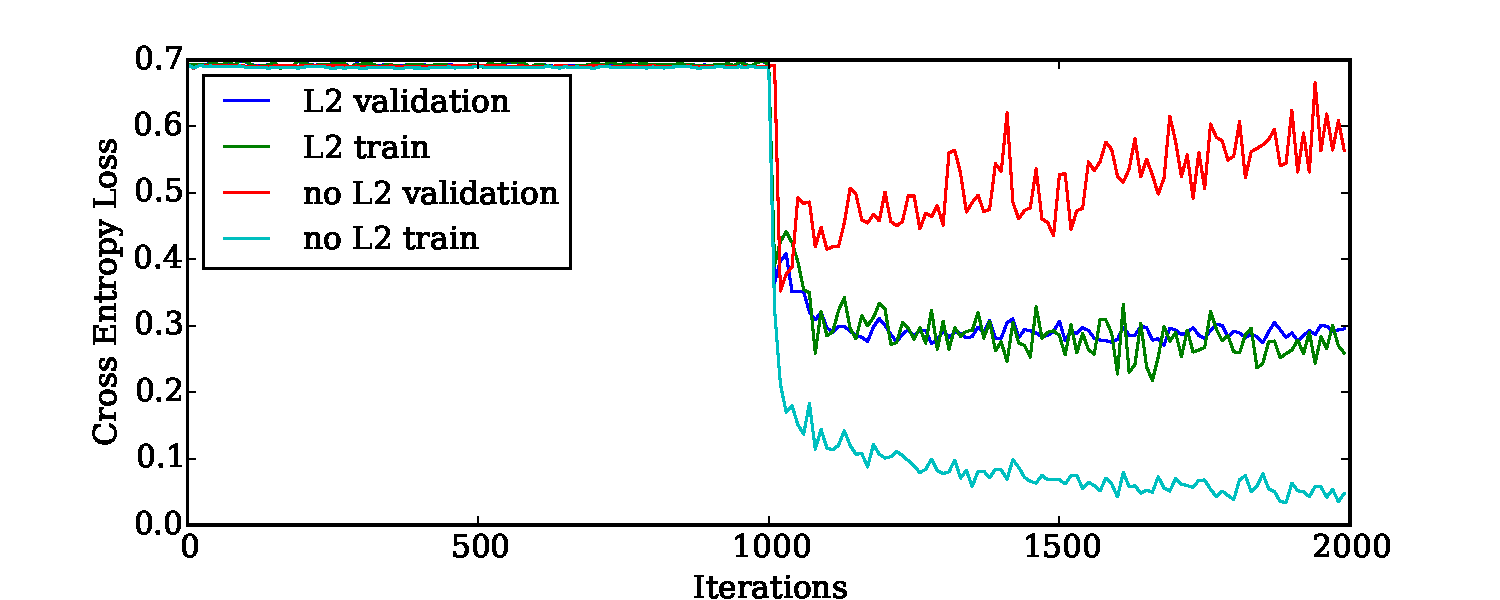
\includegraphics[width =0.8\hsize]{figures/l2.pdf}
    \caption{Plot of the classifier losses of the experiments in table \ref{tab:l2_2} }
    \label{fig:l2_1}
    \end{figure}

    \begin{figure}[!h]
    \centering
    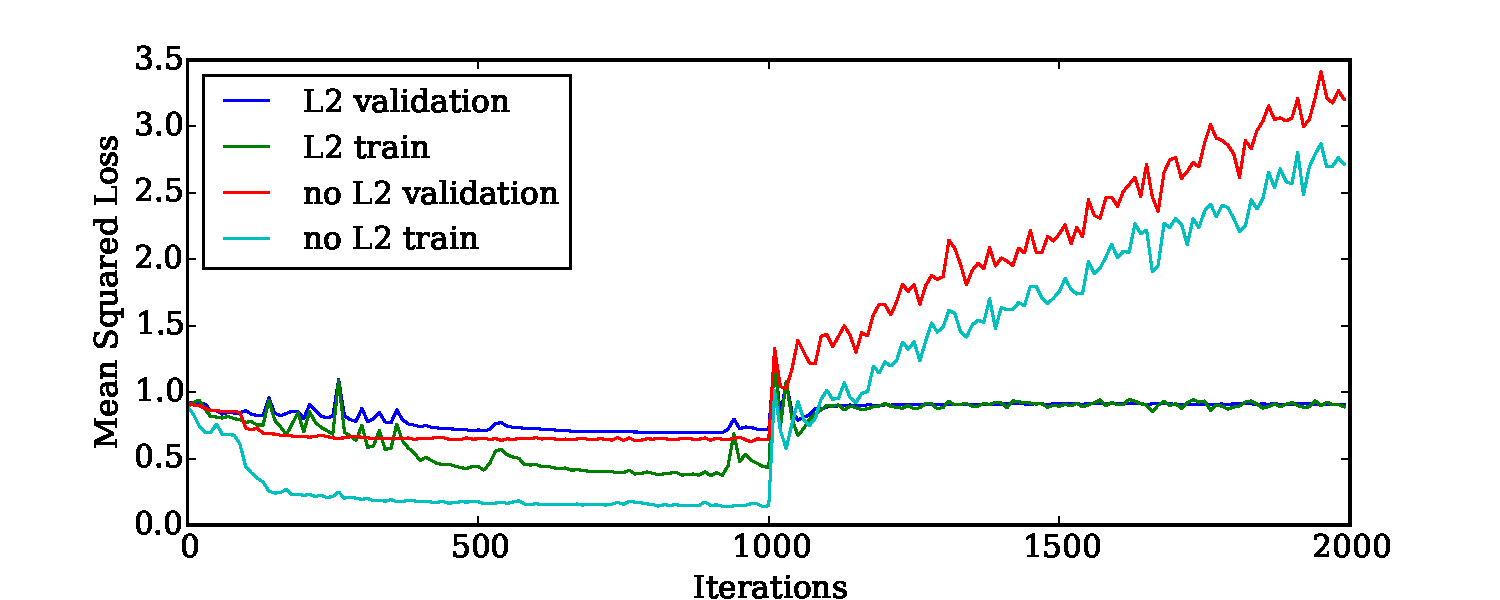
\includegraphics[width =0.8\hsize]{figures/l2_auto.pdf}
    \caption{Plot of the autoencoder losses of the experiments in table \ref{tab:l2_2} }
    \label{fig:l2_2}
    \end{figure}

    Figures \ref{fig:l2_1} and \ref{fig:l2_2} show some stuff but lets ignore it.

    \newpage

    %
    %
    %
    %
    %
    %
    \section{Denoising autoencoders}
  %
  %
  %
  %
  %
  %
  \section{Autoencoder transfer functions}
    \begin{table}[!h] { \small \centering
    		\begin{tabular}{rrrrrrrrrrrr}
    			&&&&& &  \multicolumn{3}{|c|}{Early Model} &  \multicolumn{3}{c|}{Final Model}    \\
    			\hline
    			i  & Network & alpha      & Iterations & Early Iteration & dp  & e roc & e f1 & e auto & f roc & f f1 & f auto \\
    			\hline
           1 & 2 & constant 0.0 & 1500 &  1000 &  0.8 &    0.8  &   0.47 &     0.56 &    0.79 &   0.46 &     0.64 \\
    			 2  & 2       & constant 0.5   & 1500       & 750             & 0.8 & 0.81  & 0.48 & 0.03   & 0.8   & 0.46 & 0.03   \\
    			 3  & 2       & sigmoid    & 1500       & 1000            & 0.8 & 0.8   & 0.46 & 0.03   & 0.79  & 0.46 & 0.03   \\
    			 4  & 2       & polynomial & 1500       & 750             & 0.8 & 0.79  & 0.46 & 0.03   & 0.77  & 0.44 & 0.03   \\
    			 5  & 2       & alternate  & 1500       & 1000            & 0.8 & 0.81  & 0.46 & 0.1    & 0.82  & 0.47 & 0.12   \\
           6 & 2 & step     & 1500 &  1000 &  0.8 &    0.59 &   0.19 &     0.03 &    0.82 &   0.47 &     0.08 \\
    			\hline
           7 & 3 & constant 0.0 & 1500 &  1000 &  0.8 &    0.81 &   0.43 &     2.38 &    0.79 &   0.42 &     2.61 \\
    			 8  & 3       & constant 0.5   & 1500       & 750             & 0.8 & 0.81  & 0.46 & 0.03   & 0.81  & 0.46 & 0.03   \\
    			 9  & 3       & sigmoid    & 1500       & 1000            & 0.8 & 0.8   & 0.46 & 0.03   & 0.8   & 0.44 & 0.04   \\
    		  10  & 3       & polynomial & 1500       & 750             & 0.8 & 0.78  & 0.45 & 0.02   & 0.79  & 0.44 & 0.03   \\
    			11  & 3       & alternate  & 1500       & 1000            & 0.8 & 0.69  & 0.32 & 0.1    & 0.77  & 0.37 & 0.23   \\
          12 & 3 & step     & 1500 &  1000 &  0.8 &    0.38 &   0.19 &     0.03 &    0.81 &   0.45 &     0.18 \\
    			\hline
          13  & 4       & constant 0.0   & 1500       &  1000           & 0.8  &    0.78 &   0.38 &    16.31 &    0.78 &   0.39 &    14.5 \\
    			14 & 4       & constant 0.5   & 1500       & 750             & 0.8 & 0.73  & 0.33 & 0.03   & 0.75  & 0.36 & 0.03   \\
    			15 & 4       & sigmoid    & 1500       & 1000            & 0.8 & 0.74  & 0.36 & 0.03   & 0.74  & 0.36 & 0.03   \\
    			16 & 4       & polynomial & 1500       & 750             & 0.8 & 0.52  & 0.21 & 0.09   & 0.67  & 0.3  & 0.04   \\
    			17 & 4       & alternate  & 1500       & 1000            & 0.8 & 0.6   & 0.26 & 0.06   & 0.61  & 0.27 & 0.07   \\
          18 & 4       & step       & 1500       &  1000           & 0.8  &    0.42 &   0.19 &     0.03 &    0.77 &   0.4  &     0.7 \\


    			\hline
    		\end{tabular}  } \caption{} \label{tab:pseaafasfrch} \end{table}

        Autoencoer loses are quite different between experiments, does this suggest that
        most of the logic is in the softmax layer??

        Describe alternative more complicated situations where ony hte softmax bit gets trained.


    \newpage
    %
    %
    %
    %
    %
    % \section{Comparison to classifier only network}
    % \begin{table}[!h] {\small
    %   \centering
    %   \begin{tabular}{llrrrrrr}
    %      & &   \multicolumn{3}{|c|}{Early Model} &  \multicolumn{3}{c|}{Final Model}\\
    %      \hline
    %      Preprocesing       & Activation Function&  ROC    &      F1&  AE Loss & ROC     &     F1 &   AE Loss \\
    %      \hline
    %      Per Subject Face   & linear             &    0.79 &   0.45 &     0.61 &    0.79 &   0.46 &     0.75 \\
    %      \hline
    %   \end{tabular}
    % \caption{A repeat of experiment 13 from \ref{tab:psearch} but $\alpha(t)=0$ through out.
    % It shows a slightly lower ROC score and much higher autoencoder loss, as expected because it is not training
    % the autoencoder.} \label{tab:psearchtest}}
    % \end{table}

    \newpage
    %
    %
    %
    %
    %
  % \section{Data balancing}
  %   pass
